%The \introduction command is provided as a convenience.
%if you want special chapter formatting, you'll probably want to avoid using it altogether
		
\chapter*{Introduction}
    \addcontentsline{toc}{chapter}{Introduction}
		\chaptermark{Introduction}
		\markboth{Introduction}{Introduction}
% The three lines above are to make sure that the headers are right, that the intro gets included in the table of contents, and that it doesn't get numbered 1 so that chapter one is 1.
The study of pattern formation is incredibly diverse and certainly one of the most compelling aspects of nonlinear phenomenology. Scientists from many disciplines study pattern formation on scales ranging from that of the entire universe all the way down to the microscopic.\footnote{See the introduction of Cross \& Greenside for an overview of the study of pattern formation\rf{cross_greenside_2009}.} Just a cursory glance at the structure of a wind-swept sand dune, a snowflake, or even our own spiral galaxy reveals something interesting. Observation of these patterns might lead a scientist to ask what causes the pattern and wonder why there are patterns at all. This question gets complicated quickly because whether you see `God in the patterns' or see them as the result of a non-equilibrium universe, there is still the question of what it means to have ``structure'' or ``complexity'' or even to be ``interesting''.
%
\begin{figure}[h]
	\centering
	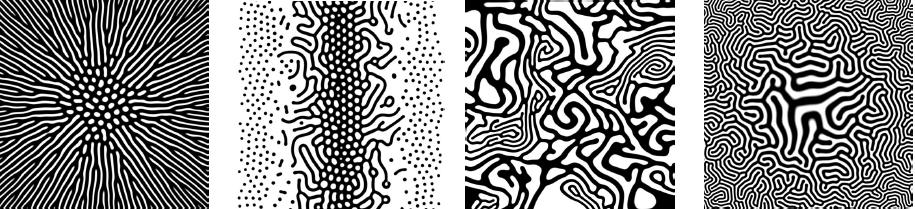
\includegraphics[width=\textwidth]{rd_examples.png}
	\caption{Patterns of the Gray-Scott reaction-diffusion system simulated by Karl Sims. Figure adapted from \protect\bibentry{karlsims}.}
	\label{fig:karl_sims}
\end{figure}

	Of course, patterns in nature are inherently difficult to understand; they are often inhomogeneous, subject to many unknown forces, or simply too large or small to study carefully. So before arriving at conclusions about the structure of the universe, it is helpful to look at idealized systems. This can mean a tightly controlled experimental setup\rf{kurtuldu_2011} or a completely computational model like the one discussed here. Indeed, the vast amount of literature on the study of pattern formation looks to these simplified, yet no less dazzling, ``prepared patterns'' to draw conclusions about natural patterns\rf{cross_greenside_2009}. One heavily studied example is Rayleigh-B\'{e}nard convection, the experimental setup for which is extremely accessible; a horizontal plane of fluid is heated from below and cooled from above which gives rise to patterns like the one shown in \refFig{fig:rbconvec}.
%
\begin{figure}[h]
	\centering
	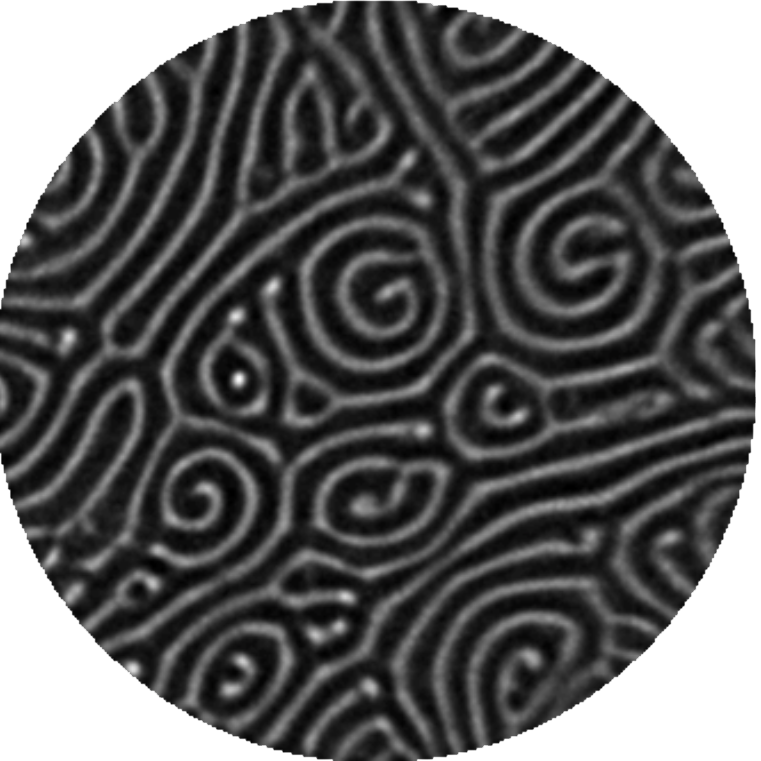
\includegraphics[width=0.3\textwidth]{rbconvec.png}
	\caption{An image of the ``prepared pattern'' formed by Rayleigh-B\'{e}nard convection. A horizontal plane of fluid is heated from below and cooled from above. Dark regions indicate the hot upflows and bright regions indicate cold downflows. Figure adapted from \protect\bibentry{kurtuldu_2011}.}
	\label{fig:rbconvec}
\end{figure}
%

	The study of patterns often comes down to the study of \textit{image data}, especially in the setting of a computational simulation. There are many mathematical tools available to help interpret this kind of data but as the complexity of our information (i.e.\ the amount of data) increases, it becomes increasingly difficult to parse relevant information.  Technological development in recent years not only makes capturing massive amounts of data possible, but commonplace. In the world of medical imaging, for example, data sets of X-Ray tomography, which allow for 3D reconstruction of biological structures such as the heart or lungs, can easily exceed dozens of gigabytes. While the increasing availability of data would serve only to improve our understanding of these systems, it is only as useful as our analytical methods allow. Traditional techniques may fall flat in the face of exceedingly sophisticated information.
	
\begin{figure}[h]
        \centering
        \begin{subfigure}[b]{0.35\textwidth}
        	\centering
                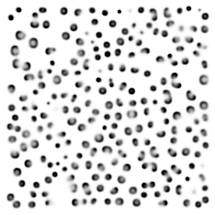
\includegraphics[width=0.85\textwidth]{alpha_v_grey.png}
                \caption{Pattern type $\alpha$.}
                \label{fig:alphagrey_fft}
        \end{subfigure}
        \begin{subfigure}[b]{0.35\textwidth}
        	\centering
                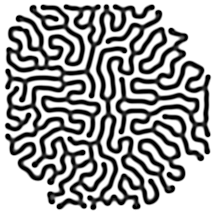
\includegraphics[width=0.85\textwidth]{kappa_v_grey.png}
                \caption{Pattern type $\kappa$.}
                \label{fig:kappagrey_fft}
        \end{subfigure} \\
        
        \begin{subfigure}[b]{0.35\textwidth}
        	\centering
                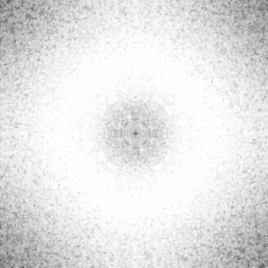
\includegraphics[width=0.85\textwidth]{alpha_v_fft.png}
                \caption{Fourier Transform of $\alpha$.}
                \label{fig:alphafft}
        \end{subfigure}
        \begin{subfigure}[b]{0.35\textwidth}
        	\centering
                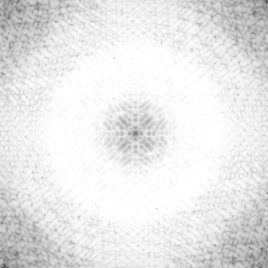
\includegraphics[width=0.85\textwidth]{kappa_v_fft.png}
                \caption{Fourier Transform of $\kappa$.}
                \label{fig:kappafft}
        \end{subfigure}
        \caption{Two very distinct pattern types of the Gray-Scott reaction-diffusion system, $\alpha$ and $\kappa$ (described further in \refSect{sect:gsmodel}). The Fourier transform of each pattern is hard to distinguish by eye and extracting meaningful information is difficult. The problematic nature of this method motivates our need for other, perhaps lower-level, analytic techniques.}\label{fig:fourierfail}
\end{figure}

	Take for example the Fourier transform, a powerful method for analysis which is often used to remove noise or apply filters to images. We would expect the Fourier transform to provide some insight into the spatial frequency of the image\footnote{In this case, the Fourier transform converts from the \textit{spatial domain}, the image we see, to the \textit{frequency domain}. The FT has been used for intricate pattern recognition, see\rf{hui_2014}.}, but in some cases, this method fails to provide useful information. Examine the two distinct pattern types of the Gray-Scott reaction-diffusion system shown in \refFig{fig:fourierfail} (more about this system in \refSect{sect:gsmodel}). The two pattern types $\alpha$ and $\kappa$ (\refFigs{fig:alphagrey_fft}{fig:kappagrey_fft} respectively) are easy to differentiate by eye yet the Fourier transforms (\refFigs{fig:alphafft}{fig:kappafft}) are disappointingly similar. Although this method is capable of extracting useful information, we would like some way to supplement our findings. The need for new methods arises and many times that means starting at the lowest level (\ie the structures that make up the image) especially when the crucial information is geometric in nature.
	
	But for many systems, it doesn't make sense to attempt to describe basic geometric structures in terms of the underlying mathematical equations (assuming we can write them down in the first place). This problem calls for a framework that gets at the geometric information even when face with numerical error and minor perturbations. The theory of computational homology described in \refChapter{ch:homology} does just this. Under the umbrella of algebraic topology, homology provides a beautiful framework for transforming topology into algebra from which one can draw insight into global properties. Although homology has only recently been brought to the fore of experimental physics, its application has shown interesting results\rf{kaczynski_2007,mischaikow_2002,gameiro_2004,mischaikow_2006}. This project explores the application of this theory to one pattern forming system in particular and highlights the information that may be derived from it.
	
	
	
	
	
	